\part{Método}

\chapter[Método]{Método}\label{Capitulo4}

\section{Processo de software}

O processo de desenvolvimento de software é algo complexo devido a variáveis que podem ter diferentes perspectivas de resultados.
Por isso é preciso definir soluções que atendam o objetivo do cliente de forma concisa. 
Aplicamos a metodologia ágil do Scrum, que nos ajudou na agilidade do processo de software, definindo as ações em cada atividade, a saber: (i) levantamento de requisitos, (ii) implementação do sistema e (iii) implantação do sistema.

Optamos por uma metodologia ágil, que é mais indicada para cenários como o nosso, equipe pequena e prazo curtos.
Com ela pudemos aplicar um fluxo de forma mais ágil, levantamos os requisitos, identificamos os problemas e definimos as soluções.
Em seguida, documentamos essas soluções através dos casos de uso e iniciamos a implementação, adotando as tecnologias e arquitetura com as quais temos mais experiência.

\section{Levantamento de requisitos}

Através do levantamento de requisitos deterinamos o problema.
Essa identificação foi feita através de reuniões com o setor de compras do IFG câmpus Formosa, em que resumimos os seguintes tópicos:

\begin{itemize}
    \item Descentralização das informações necessárias.
    \item Problemas de comunicação entre os interessados.  
    \item Problemas de comunicação na fase interna.  
    \item Problema com a solicitação de pedidos.
\end{itemize}

Com esses pontos notamos que o maior problema da fase interna era a comunicação. 
Com base nesses tópicos continuamos o levantamento de requisitos e montamos soluções hipotéticas usando casos de uso, que depois foram validados com o cliente.

\begin{itemize}
    \item O caso de uso~\ref{CASO001} mantém os dados sobre  materiais, serviços, items e licitações atualizados.
    
    \item O caso de uso~\ref{CASO002} permite ao usuário solicitar a inclusão de items e suas quantidades em uma licitação.

    \item O caso de uso~\ref{CASO003} permite que o usuário avalie o pedido de participação na licitação.
    
    \item O caso de uso~\ref{CASO004} permite que o usuário veja a resposta do pedido de participação na licitação.

\end{itemize}

%Portanto nossa solução é centralizar as informações necessárias para a participação de outros campus na licitação e melhorar a comunicação entre eles.

\section{Implementação do sistema}

Desenvolvemos o sistema usando um \textit{framework} chamado JHipster na versão 4.13.2 que gera o esqueleto da aplicação, deixando pronta todo um \textit{front-end} básico, o \textit{back-end}, a comunicação entre entre eles e a integração com o banco de dados.

%E com isso conseguimos agilizar o processo desenvolvimento da aplicação web pois o ambiente de desenvolvimento foi montado de forma rápida e 

Utilizamos a API de compras governamentais para buscar as informações necessárias sobre items, materiais, serviços e licitação.
Estes dados são então salvos no nosso banco de dados.

A implementação da aplicação foi baseada em uma \textit{stack} (pilha) de programas.
Para o desenvolvimento da estrutura lógica do sistema e integração com o banco de dados utilizamos JPA na versão 2.1 e o Hibernate na versão 5.2.12. Utilizamos \textit{Spring boot} na versão 1.5.9 para auxiliar no desenvolvimento criando uma API com arquitetura REST para a comunicação com o front-end.
Os dados foram persistidos no SGBD MySQL na versão 5.7 conforme o modelo de dados mostrado na~\ref{Figura007}.

\begin{sidewaysfigure}[ht]
	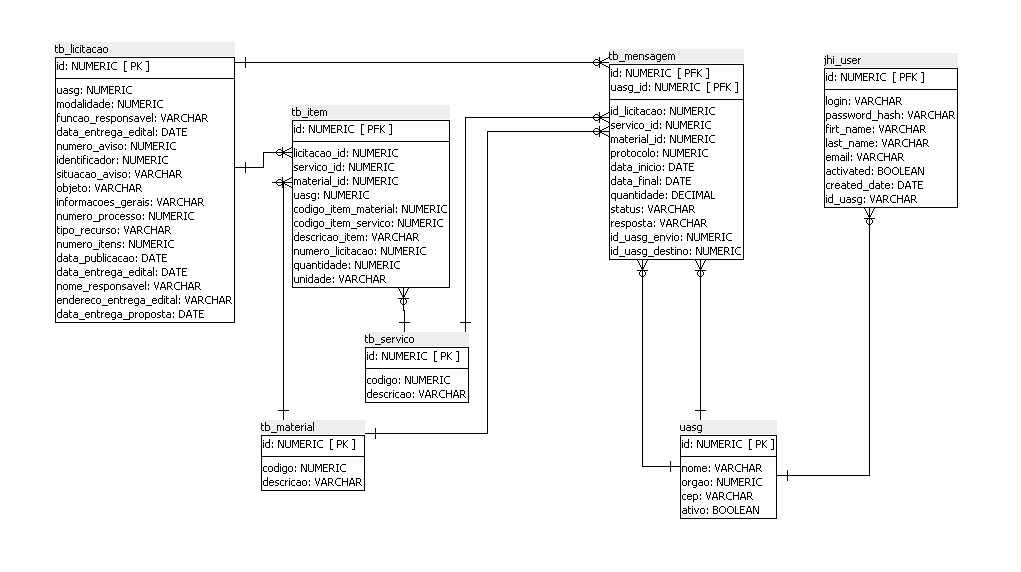
\includegraphics[width=0.95\textwidth]{figuras/bdAtualizado.png}
	\caption{Modelo de dados do projeto.}
	\label{Figura007}
\end{sidewaysfigure}

Como o sistema é Web, o front-end foi criado utilizando  HTML e CSS, auxiliados por \textit{scripts} JavaScript para dar dinamismo na forma de apresentação de dados.
O AngularJS na versão 1.x auxiliou no desenvolvimento estabelecendo a comunicação entre o \textit{front-end} e o \textit{back-end}, além da criação das rotas do sistema.
Na estilização da tela usamos componentes \textit{on demand} do \textit{framework} O Bootstrap.

A arquitetura do nosso sistema é apresentada da~\prototipo{Figura005}.
O \textit{front-end} realiza chamadas de método para o \textit{back-end}, o qual as processa, se for o caso busca os dados no banco de dados, e retorna-os para o front-end.
O \textit{front-end} depende do \textit{back-end} apenas para os dados, mantendo-se visível ao usuário, idependente da ação.

\begin{sidewaysfigure}[ht]
    \centering
    \includegraphics[width=0.95\textwidth]{figuras/figura005.png}
    \caption{Arquitetura do projeto.}
    \label{Figura005}
\end{sidewaysfigure}

\section{Implantação do sistema}

A implantação do sistema ainda não ocorreu.
A implanatação é agora dependente do cliente, o qual deverá proporcionar aos desenvolvedores uma agenda para a avalidação das soluções implementadas.